\documentclass[11pt]{article}
\usepackage[margin=2.15cm]{geometry}
\usepackage{graphicx}
\usepackage{booktabs}
\usepackage{microtype}
\usepackage[numbers,sort&compress]{natbib}
\usepackage[hidelinks]{hyperref}
\usepackage{xcolor}
\usepackage{authblk}
\usepackage{lineno}
\usepackage{caption}
\usepackage{enumitem}
\definecolor{navy}{HTML}{173B57}
\definecolor{blocked}{HTML}{9B2C2C}
\captionsetup{font=small,labelfont=bf}
\setlength{\parindent}{0pt}
\setlength{\parskip}{0.48em}
\emergencystretch=1em
\linenumbers

\title{\textbf{Replay-bound virtual chemistry reveals hidden failure modes in autonomous experimental agents}}
\author{\textbf{AUTHORS AND AFFILIATIONS TO BE FINALIZED}}
\date{Nature Article submission draft, 12 July 2026\\
\textcolor{blocked}{Rendered for author review; full benchmark evidence and submission metadata remain incomplete}}

\begin{document}
\maketitle

\begin{abstract}
Agents that automate scientific experiments must choose measurements, act under safety and cost constraints, and revise decisions from incomplete evidence. Existing chemical evaluations emphasize static knowledge, a single optimization surface or costly physical laboratories, making it difficult to separate algorithmic adaptation from scaffolding and simulator artifacts. Here we introduce ChemWorld, a replay-bound virtual chemistry environment that exposes classical optimizers, reinforcement-learning policies and tool-using language models to one typed experimental contract. Six research tasks combine reaction, separation, flow, electrochemical and equilibrium operations with hidden executable mechanism families. A layered evaluator recomputes primary endpoints, risk, cost, validity, interaction capability and method resources from trajectories. In a pre-registered four-task confirmation, safety-constrained Gaussian-process optimization reduced risk and cost and improved every primary endpoint relative to random search, but missed the flow-task smallest effect of interest (0.018752 versus 0.020000), causing the joint rule to fail. Development diagnostics further show that lowering risk confidence did not improve this frontier and that a 100,000-step SAC run regressed after its 80,000-step checkpoint. Nine mechanism-family controls were detectable, bounded and mass conserving, but agent adaptation to them remains untested. ChemWorld therefore provides an auditable substrate for studying closed-loop scientific decision-making while explicitly separating implemented controls from claims that still require multi-seed, live-model, hidden-world and independent-reproduction evidence.
\end{abstract}

\section*{Main}

Scientific autonomy is not chemical recall. An experimental agent must allocate a finite budget, select operations and instruments, interpret partial observations, respond to invalid or unsafe states and apply earlier experience to later experiments. Physical self-driving laboratories have demonstrated closed-loop reaction and materials optimization \citep{shields2021bo,szymanski2023alab,abolhasani2023sdl}; language-model systems can plan procedures and invoke chemistry tools \citep{boiko2023coscientist,bran2024chemcrow}. These systems establish feasibility, but their hardware, orchestration and resource costs differ enough that an apparent model improvement can instead reflect an easier interface, more measurements or hidden human assistance.

Static chemistry benchmarks provide complementary evidence about knowledge and reasoning \citep{jablonka2024predictive,schneider2024chembench}. ScienceAgentBench extends evaluation to executable data-driven research tasks and shows the need to measure both outcome and cost \citep{chen2025scienceagentbench}. Embodied laboratory simulation is also advancing: ChemGymRL provides connected virtual chemistry benches \citep{beeler2024chemgymrl}, and LabUtopia combines procedural laboratory scenes with hierarchical manipulation tasks \citep{li2025labutopia}. ChemWorld addresses a different layer of the problem. It asks whether heterogeneous agents can be compared under the same partially observable, multi-experiment chemical decision contract, and whether that contract can later support training without confusing success in a simulator with transfer to reality.

\subsection*{A common contract for heterogeneous agents}

ChemWorld separates the agent, public interface, hidden world, evaluator and evidence layer (Fig.~\ref{fig:system}). The public interface exposes only task goals, legal operations, released measurements, resource state and prior public history. Actions are typed and validated before execution. The hidden world owns state, mechanisms, constitutive laws, instrument noise and world-family shifts. The evaluator is read-only: it replays the trajectory and recomputes endpoint, constraint and resource quantities rather than trusting a submitted score.

The separation matters because the compared methods act at different temporal scales. Recipe-search methods select a complete experimental recipe and update between experiments. Operation-open-loop agents emit an operation sequence without using intermediate evidence. Operation-closed-loop agents can change the next operation after each measurement. ChemWorld records these capability strata but does not collapse them into the endpoint score. Cross-stratum comparisons describe complete systems; algorithm-only attribution requires the same interaction and information contract.

Trajectories contain concise public evidence, hypothesis, uncertainty and rationale fields where an agent provides them. They do not require or score private chain-of-thought. Online language models additionally retain provider and model identity, prompt digest, request parameters, token usage, cost, retries and failures. The benchmark harness does not silently repair a failed model action, terminate an experiment or perform a final assay on the model's behalf.

\begin{figure}[t]
  \centering
  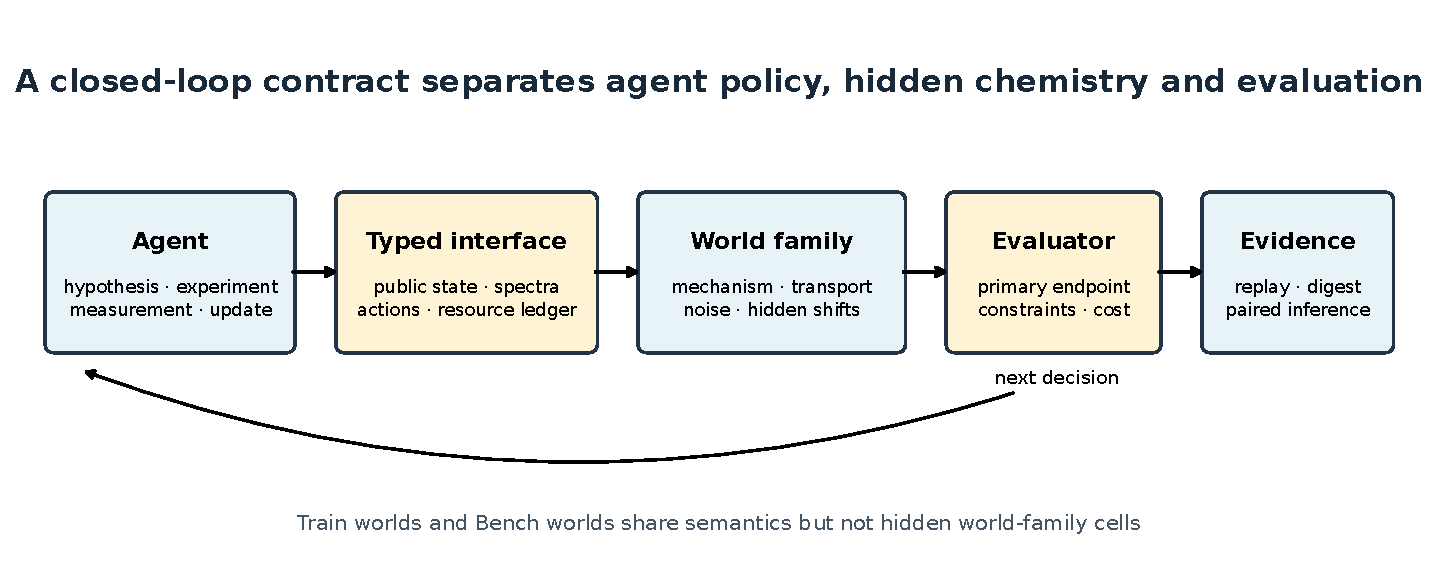
\includegraphics[width=\textwidth]{figures/figure1_system.pdf}
  \caption{\textbf{Replay-bound architecture for closed-loop virtual chemistry.} Agents interact only through a typed public contract. Hidden world families alter executed mechanism and observation models without changing public task semantics. Endpoint, risk, cost, validity, interaction and resource quantities are recomputed from trajectories and bound to source records by digests.}
  \label{fig:system}
\end{figure}

The environment currently registers fifteen task slices. Six research tasks span liquid--liquid partition, reaction--crystallization, reaction--distillation, continuous-flow reaction optimization, electrochemical conversion and equilibrium characterization. Four form a provisional comparison core; electrochemistry and equilibrium remain exploratory because their declared primary capabilities have not yet passed the same empirical-validity rule. Registered software functionality is therefore not equated with benchmark validity.

\subsection*{Objective-only optimization hides operational risk}

The initial structured Gaussian-process diagnostic improved the declared primary endpoint on partition, crystallization, distillation and flow reaction. A layered reanalysis changed the interpretation: risk-budget exceedance increased by 16.0, 27.3 and 39.0 percentage points for flow, crystallization and distillation, respectively, relative to random search. Partition improved by 7.3 percentage points. All four cost rules passed, but three safety rules failed. Thus, a method that appeared uniformly superior under objective-only reporting was unacceptable under the joint endpoint--risk--cost rule.

This failure motivated a constrained policy rather than a change to the score. Safe-GP models the maximum operational risk observed during each complete experiment, begins from a conservative public design, represents material choices categorically and filters candidate recipes by an upper-confidence risk bound. Its implementation, recipe space, task-specific smallest effects of interest (SESOIs), constraint margins and paired analysis were frozen before a separate confirmation.

The confirmation contained four tasks, three methods, twenty paired worlds and forty complete experiments per task--method--world cell (240 trajectories and 9,600 experiments). Every trajectory passed a second replay and metric recomputation. Safe-GP reduced risk exceedance and experiment cost relative to random search on every task (Fig.~\ref{fig:safegp}b). Its primary endpoint effect was positive for all four tasks (Fig.~\ref{fig:safegp}a). Partition, crystallization and distillation exceeded their SESOIs. Flow reaction produced a mean paired effect of 0.018752 (paired interval 0.013144--0.023698), below the pre-registered SESOI of 0.020000. Because the rule was conjunctive, the complete comparison failed despite passing eleven of twelve task-level objective, risk and cost components.

\begin{figure}[t]
  \centering
  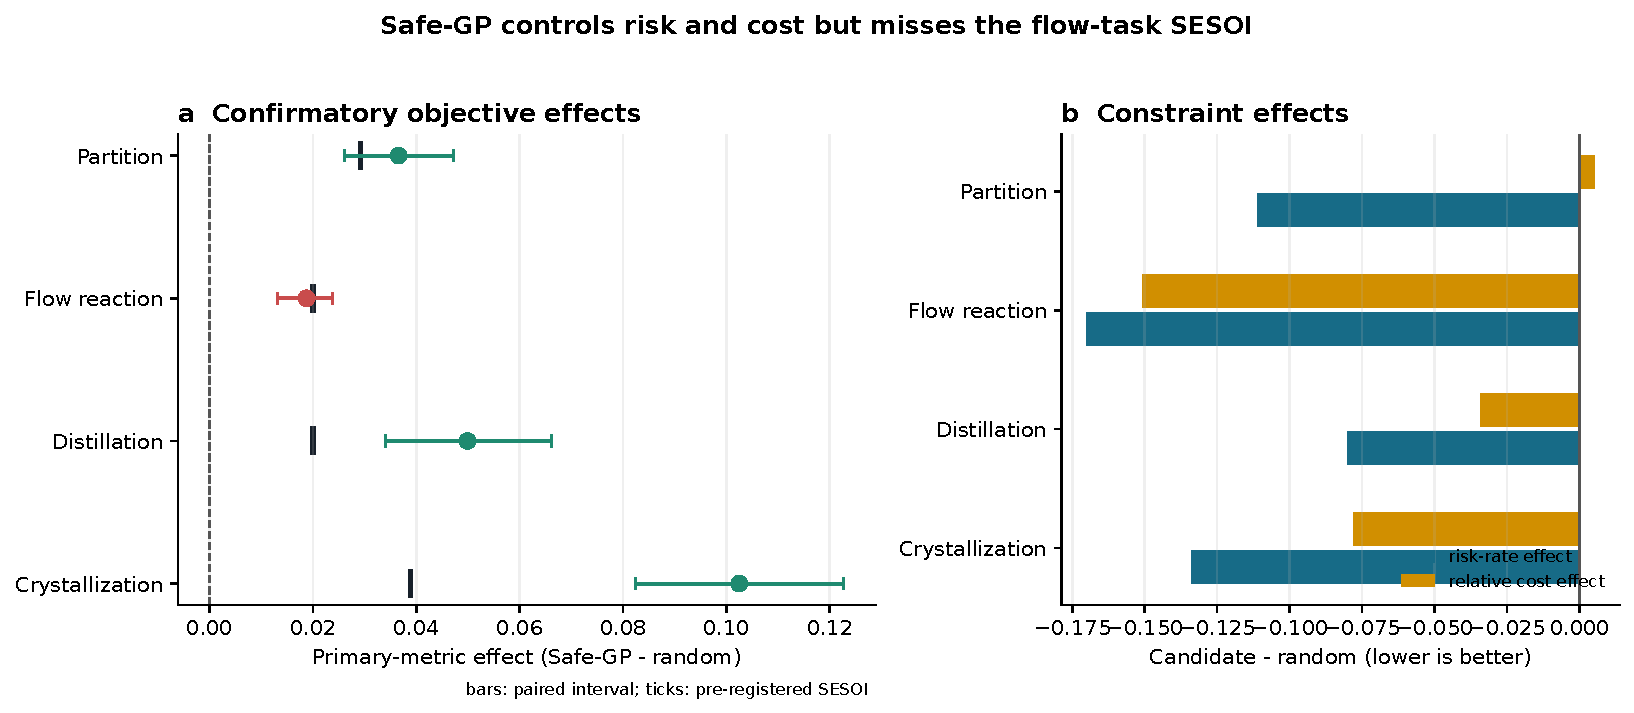
\includegraphics[width=0.98\textwidth]{figures/figure2_safe_gp_confirmatory.pdf}
  \caption{\textbf{A safety-constrained optimizer improves all endpoints but fails the joint rule.} \textbf{a}, Paired Safe-GP-minus-random effects on declared primary metrics; bars are paired intervals and vertical ticks are task-specific SESOIs. Red marks the failed flow-task joint decision. \textbf{b}, Mean paired changes in risk-budget exceedance rate and experiment cost; negative values favour Safe-GP. The slice contains twenty paired worlds per task.}
  \label{fig:safegp}
\end{figure}

The result is scientifically useful precisely because it is not upgraded to a win. It exposes a boundary at which statistical direction, operational constraints and practical effect size disagree. It also prevents repeated tuning on the confirmation cohort: any structural policy revision requires a new development cohort and another untouched confirmation.

\subsection*{Development diagnostics reject simple improvement heuristics}

We next asked whether the flow miss reflected an overly conservative risk coefficient. A post-confirmatory development diagnostic compared the frozen risk-confidence coefficient $\beta=2.0$ with $\beta=1.5$ and $\beta=1.0$ on five new worlds. Each method completed forty experiments per world and all trajectories replayed. The incumbent $\beta=2.0$ obtained the highest mean flow conversion (0.05756), lowest risk exceedance rate (0.020) and lowest mean cost per experiment (0.39776). Both lower coefficients had negative paired objective effects relative to the incumbent and cost regression exceeding 5\%. Lowering $\beta$ therefore did not produce a better objective--risk--cost frontier (Fig.~\ref{fig:diagnostics}b). This small diagnostic rejects a simple repair; it does not validate the incumbent or overwrite the failed confirmation.

Reinforcement learning exposed a parallel failure of a common heuristic. A Soft Actor--Critic development run completed exactly 100,000 environment steps on the flow task, with model and replay-buffer checkpoints every 20,000 steps. Training produced 19,504 complete experiments. Evaluation episodes were complete and nearly free of invalid actions; ten standard trajectories replayed exactly. However, the mean episode-best development score peaked at 0.023782 after 80,000 steps and fell to 0.010552 at 100,000 steps (Fig.~\ref{fig:diagnostics}a), a 55.6\% regression. The final budget is therefore not a defensible default checkpoint. Pooled selection across multiple training seeds is required before formal RL evaluation.

\begin{figure}[t]
  \centering
  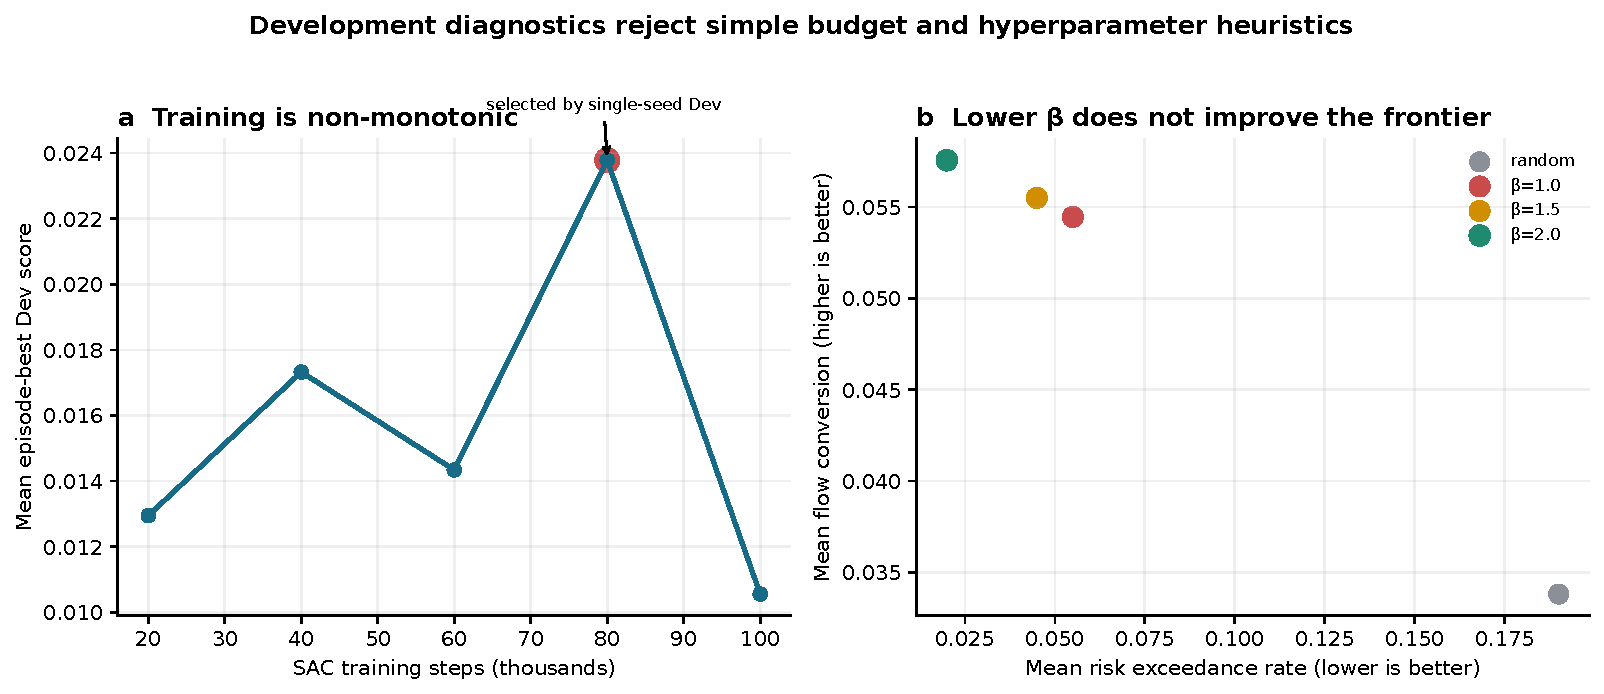
\includegraphics[width=0.96\textwidth]{figures/figure3_development_diagnostics.pdf}
  \caption{\textbf{Development diagnostics falsify simple tuning heuristics.} \textbf{a}, Single-seed SAC development score across exact training checkpoints; the 100k checkpoint regresses from the 80k maximum. \textbf{b}, Five-world Safe-GP risk--conversion trade-off; marker size also reflects experiment cost. Lowering the confidence coefficient does not dominate the frozen policy. These panels are development evidence, not formal method comparisons.}
  \label{fig:diagnostics}
\end{figure}

Together, these diagnostics show why an agent gym needs more than a terminal score. Experiment count, training steps, candidate evaluations, decision time, process CPU, model calls and monetary cost are different resources. ChemWorld retains them separately and reports performance as task-specific frontiers rather than a universal scalar leaderboard.

\subsection*{Executable mechanism families make adaptation falsifiable}

A virtual training environment is vulnerable to shortcut learning: an agent may exploit a simulator artifact that is stable within the benchmark but absent from the intended phenomenon. Random seeds alone do not test this failure because they can change noise while preserving the same causal law. ChemWorld therefore exposes hidden, versioned intervention families only through providers that execute the changed law.

Reaction--crystallization, reaction--distillation and continuous flow support rate-law and topology families derived from their compiled reaction networks. Partition uses an activity-corrected constitutive exponent. Electrochemistry changes the standard-potential, transfer-coefficient and overpotential--selectivity response used by its Nernst--Butler--Volmer provider. Equilibrium changes the activity-coefficient ratio inside the weak-acid charge-balance solver. Constitutive interventions do not rewrite an unrelated reaction network.

Each of the nine task--mode combinations was calibrated with five worlds and five representative recipes (25 paired responses). A control passed only if the median absolute score change exceeded 0.005, at least half of responses were detectable, the 90th-percentile absolute change did not exceed 0.15, the transformation was deterministic and mass balance remained within $10^{-8}$. All nine combinations passed (Fig.~\ref{fig:mechanisms}). Public trajectories retain only an opaque intervention version and hash; exact intervention context is supplied out of band for replay, and missing or altered context fails closed.

\begin{figure}[t]
  \centering
  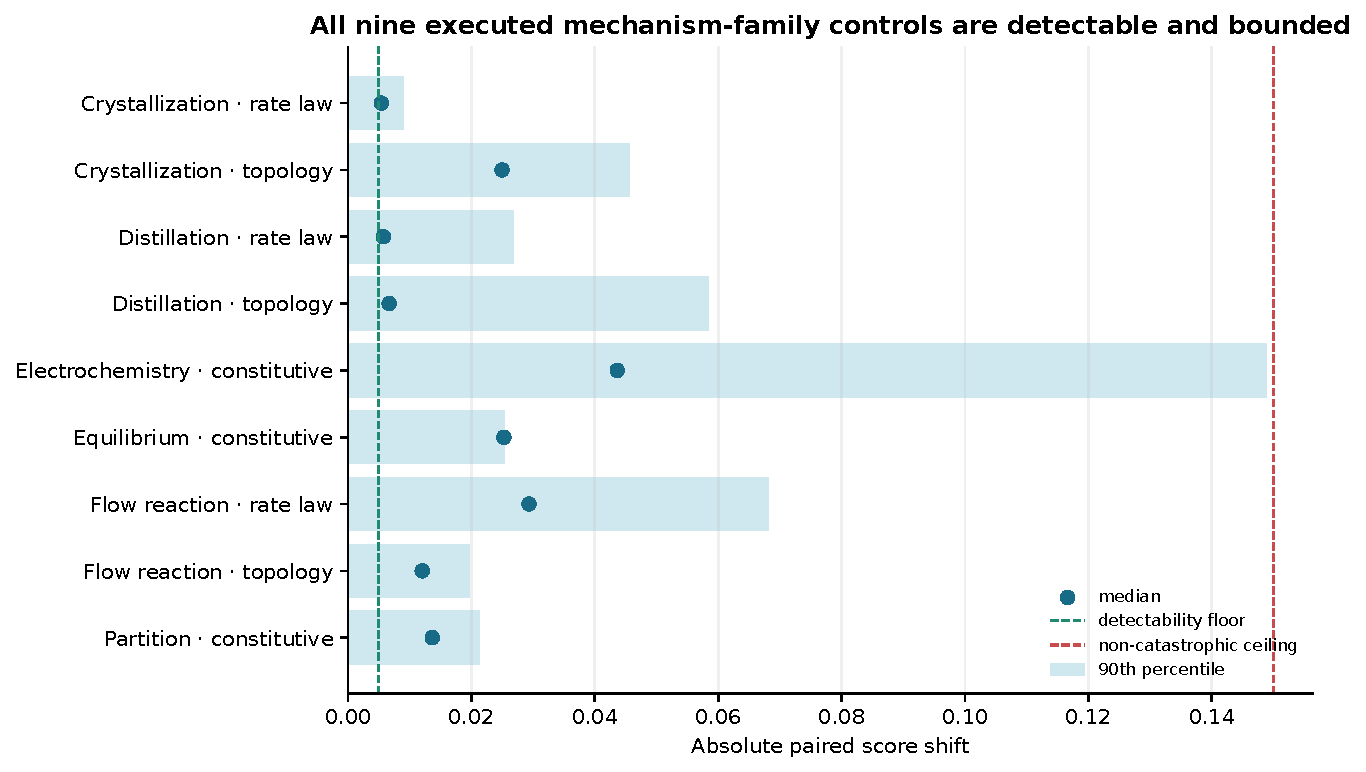
\includegraphics[width=0.82\textwidth]{figures/figure4_mechanism_controls.pdf}
  \caption{\textbf{Executed mechanism-family interventions are detectable and bounded.} Bars show the 90th percentile and points the median absolute paired score shift across 25 world--recipe probes. Dashed lines mark the predeclared detectability floor and non-catastrophic ceiling. All combinations also passed determinism and mass-balance checks. These controls validate the environment intervention, not agent identification or transfer.}
  \label{fig:mechanisms}
\end{figure}

This design turns the training-environment question into an experiment. Agents can be trained on allocated families, selected on disjoint development cells and evaluated once on unseen Bench families. The claim-changing endpoint is not high reward in simulation but an equal-budget advantage over training from scratch on unseen virtual or external bridge tasks. That experiment has not yet been completed.

\subsection*{Spectra and model reasoning require causal controls}

ChemWorld instruments return state-coupled synthetic HPLC, GC, UV--visible, infrared, NMR, mass-spectrometry, pH and final-assay packets. Operation-level language-model adapters receive a compact public context and can update after every measurement. The paired spectral protocol compares an assigned condition with a masked condition on identical task, world, budget and model seed. Masking removes spectra, chromatograms, peaks, channels and assignments while retaining endpoints, mass balance, cost, constraints and budget. This differential control is needed because deleting an entire measurement packet would confound spectral information with other evidence.

The frozen online roles use DeepSeek V4 Pro in thinking mode and V4 Flash in non-thinking mode. The provider client records cache-hit and cache-miss input tokens, output tokens, calls, retries, failures, access date and a frozen price snapshot. Private chain-of-thought is neither requested for the benchmark record nor retained; structured public evidence and rationale are sufficient for trace audit. These controls pass fake-client end-to-end replay, but no real provider trajectory is present. We therefore make no statement about language-model performance or the value of spectra to a live model.

\subsection*{Engineering controls are not scientific validation}

The global architecture audit requires every control and every formal evidence component to pass independently. Implemented controls currently cover task validity, world-family axes, mechanism interventions, interaction, method resources, risk and cost, semantic invariance, public messaging, exploit probes, replay, reference-regret protocol, RL substrate, live-model adapter and confirmatory freezing. The formal layer additionally requires completed cross-method results, task confirmation, mechanism adaptation, score-replay results, hidden-world security, RL and live-model matrices, independent reference search and exploit evidence. None of these formal components is yet publication-ready (Fig.~\ref{fig:gates}); eleven active scientific issues remain.

\begin{figure}[t]
  \centering
  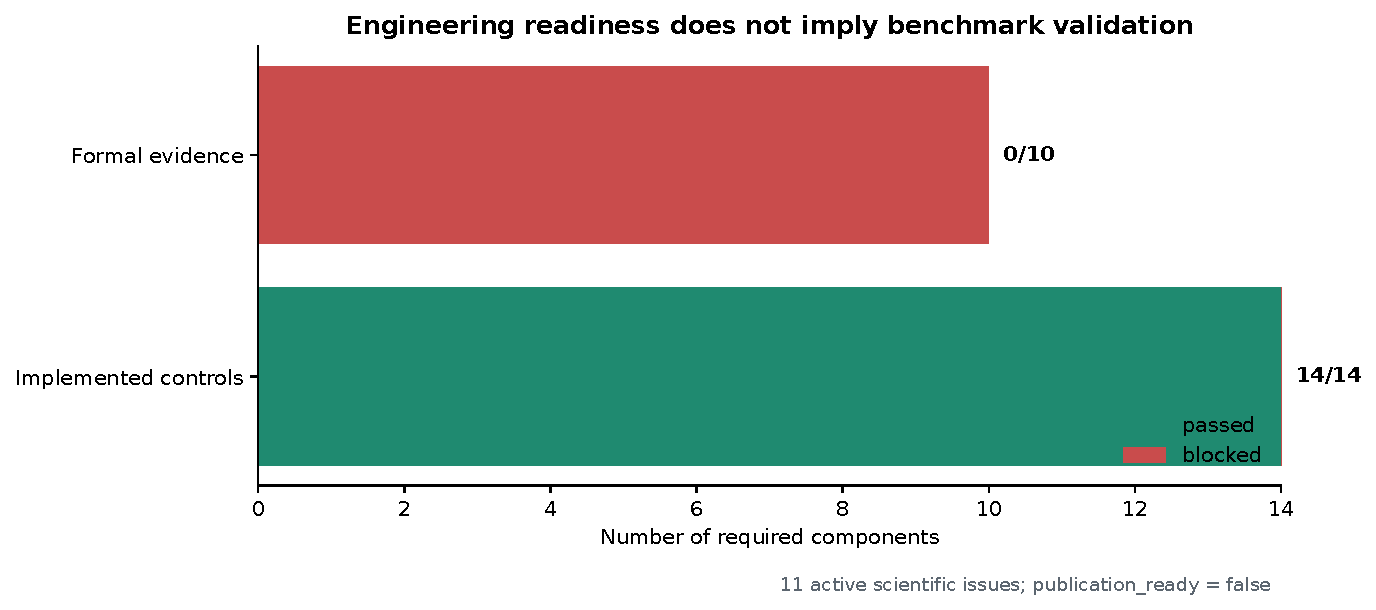
\includegraphics[width=0.83\textwidth]{figures/figure5_evidence_gates.pdf}
  \caption{\textbf{Passed engineering controls do not imply a validated benchmark.} The architecture audit evaluates control and formal-evidence components separately under a conjunctive release rule. All required controls are present, whereas the formal evidence layer remains blocked. Counts are generated directly from the versioned readiness report.}
  \label{fig:gates}
\end{figure}

ChemWorld is consequently best understood as an experimental instrument for studying adaptive decision-making, not as a surrogate for chemical truth. The current evidence supports the software contract, the constrained classical failure case, the RL and hyperparameter diagnostics, and the causal reachability of hidden mechanism families. It does not support a complete agent ranking, Train-to-Bench transfer, private-world generalization or prediction of physical-laboratory performance. Keeping those distinctions executable is the central contribution: claims can be upgraded only when the corresponding evidence gates are satisfied without changing the benchmark after results are observed.

\section*{Methods}

\subsection*{Environment and state transition}

ChemWorld implements the Gymnasium interface \citep{towers2024gymnasium}. A task declares its objective, primary metric, operation and instrument affordances, episode mode, experiment and operation budgets, world split and evaluation contract. State is stored in typed species, phase, vessel, equipment, thermal and process ledgers. Each action is canonicalized and validated before a domain service applies a provisional state patch. Constitution checks cover non-negative material amounts, phase aggregation, equipment ownership, volume and energy accounting. A valid patch is committed atomically; an invalid patch is rolled back and retained as a failed operation.

The public observation contains only released values and an explicit observed mask. Unmeasured array values are represented as non-finite internally and serialized as null, never as zero. Task scoring is separate from the transition reward. The final objective and declared primary endpoint are calculated from terminal assay evidence; online shaping cannot serve as score authority.

\subsection*{Campaigns and interaction strata}

A campaign contains multiple complete experiments under a cumulative operation budget. Recipe-search agents choose all operations for one experiment and update their surrogate between experiments. Operation-level agents choose one operation at a time. Each public decision context contains campaign progress, visible metrics, latest released instrument packet, uncertainty, constraint flags and currently available operations. The evaluator derives declared and observed within-experiment and across-experiment adaptation without inserting these quantities into the endpoint score.

\subsection*{Classical policies and frozen confirmation}

Classical controls include random search, Latin-hypercube sampling, local greedy search, typed Gaussian-process EI/PI/UCB, typed random-forest EI and typed risk-constrained GP. Categorical material choices use one-hot coordinates; numerical material identifiers are serialization labels and are not treated as ordinal distances.

The Safe-GP confirmation used random search, unconstrained typed GP and typed Safe-GP on partition, crystallization, distillation and flow tasks. Each method received forty complete experiments in each of twenty paired worlds. The primary comparison was Safe-GP versus random. A task passed only if the paired effect had the correct direction, passed the multiplicity-adjusted test, reached the predeclared SESOI and satisfied simultaneous non-inferiority rules for risk exceedance and relative experiment cost. The all-task decision was the conjunction of task decisions. Failed or incomplete runs would have remained in the denominator; none occurred.

\subsection*{Safe-GP failure diagnostic}

After confirmation, the confidence-coefficient diagnostic used five new development worlds and did not access the confirmation cohort. Random search and Safe-GP with $\beta \in \{2.0,1.5,1.0\}$ each received forty experiments. A revision required positive paired objective change against $\beta=2.0$, no more than five percentage points of risk-rate regression and no more than 5\% relative cost regression. Neither lower coefficient passed. The diagnostic is intentionally underpowered for a performance claim and is used only to reject the proposed revision.

\subsection*{Reinforcement-learning development run}

The SAC agent used Stable-Baselines3 2.9.0 and PyTorch 2.13.0 on CPU. Training was restricted to the flow-reaction Train allocation and requested exactly 100,000 environment steps. Model and replay-buffer checkpoints were retained every 20,000 steps with SHA-256 digests. Each checkpoint was evaluated on the same development protocol; the final 100k policy additionally used twenty development episodes and ten standardized replay episodes. Benchmark evaluation ignored shaped training reward and recomputed task endpoints from trajectories. Because only one training seed and one task are available, no formal RL comparison is reported.

\subsection*{Mechanism-family construction and calibration}

Reaction rate-law interventions change an executed Arrhenius equation family with a bounded activity factor; topology interventions add a reverse competition channel to the compiled network. Partition changes its executed distribution-coefficient exponent. The electrochemical family changes standard potential, transfer asymmetry and overpotential-dependent selectivity. The equilibrium family changes the activity coefficient ratio in the monoprotic charge-balance equation. Severity was fixed at 0.8 for the control audit. Five deterministic worlds and five recipe probes generated 25 paired base/intervention responses for each mode. Detectability and non-catastrophic thresholds were fixed before aggregation. These thresholds target benchmark identifiability and do not represent real chemical calibration.

\subsection*{Language-model adapter and spectral ablation}

The online adapter makes one JSON request per environment operation. Required public fields are action, evidence, spectral interpretation, hypothesis, uncertainty and rationale. Missing or malformed output becomes an invalid \texttt{model\_failure} action; the harness does not repair it. Assigned spectral packets include permitted public raw and processed features. Masking recursively removes spectral and chromatographic fields from composite packets while preserving non-spectral fields. Provider usage and frozen prices are accumulated across retries. No credential or real-model result was available for this manuscript.

\subsection*{Layered evaluation, replay and security}

The evaluator independently reports terminal objective, primary metric, shaping reward, risk constraints, process and measurement cost, validity, interaction diagnostics and method resources. Resource axes are not scalarized into the endpoint. Replay reloads source trajectory records, re-executes operations under the bound task, world and intervention context, checks trajectory bytes and digests, and recomputes the evaluation payload. Missing intervention context, non-finite values, score substitution or digest mismatch fails closed.

Student code communicates with the evaluator through bounded JSON messages in a separate process. This is a protocol boundary, not an operating-system security sandbox. Untrusted formal evaluation requires a separate low-privilege, no-network, resource-limited container with read-only benchmark assets.

\subsection*{Statistics and evidence generation}

Classical primary effects are paired by task and hidden world. Intervals and multiplicity decisions follow the frozen confirmation report. The Safe-GP $\beta$ and SAC checkpoint panels are descriptive development diagnostics without confirmatory intervals. Mechanism controls report median, 90th percentile and detectable fraction over paired world--recipe responses. Figures are generated from versioned JSON evidence by \texttt{scripts/build\_nature\_figures.py}; source CSV files and upstream SHA-256 values are retained in \texttt{paper/source\_data}. A claim audit checks source existence and digests, required limitation language, blocked-claim exclusion and rendered PDF presence.

\section*{Limitations}

ChemWorld is a virtual environment and has not been shown to preserve agent rankings in a physical laboratory. Four tasks form only a provisional comparison core; electrochemistry and equilibrium still lack a confirmed adaptive primary metric. The Safe-GP result is a bounded classical slice and fails its all-task rule. The SAC result has one model seed and one task. No eligible real language-model trajectory, mechanism-adaptation result, independent reference portfolio, salted private-world result or independent clean-install reproduction is available. Operational risk is a benchmark quantity, not a laboratory safety guarantee. The public process boundary does not safely isolate hostile code. Training-transfer and real-world claims remain prospective experiments rather than conclusions.

\section*{Data availability}

The manuscript uses versioned control, development and confirmatory-slice reports distributed with the repository. Figure source tables and a digest manifest are included in \texttt{paper/source\_data}. No physical experimental data are used. A permanent archive DOI and immutable release tag must be assigned before external submission.

\section*{Code availability}

Environment, agents, evaluators, replay verifiers, audits and manuscript-generation code are available in the ChemWorld repository. A submission must cite an immutable release rather than a mutable branch. Credentials, private salts and hidden evaluation parameters are not included in public artifacts.

\section*{Acknowledgements}

To be supplied and approved by the authors. No funding statement has been inferred.

\section*{Author contributions}

To be supplied using the CRediT taxonomy and approved by all authors before submission.

\section*{Competing interests}

To be declared by all authors before submission.

\bibliographystyle{unsrtnat}
\bibliography{references}

\end{document}
